% !TEX root = ../swputhesis.tex
\chapter{基于多聚类中心距离加权的无监督网络异常流量检测方法}
\section{引言}
随着互联网技术的飞速发展与新型网络应用的不断涌现，网络流量的规模与复杂性
呈指数级增长。面对日益复杂的网络环境，零日攻击（Zero-day Attacks）和
高级持续性威胁（APT）等未知网络攻击层出不穷。在真实网络环境中，异常流量
往往呈现出类型未知、标签稀缺甚至完全缺失的特点 。传统依赖监督信息的方法
在此类场景下适用性有限 ，因为它们通常需要大量带有精确标签的样本进行训练
，且难以泛化到模型未曾见过的攻击模式上。因此，如何在缺乏异常标签的无监督
条件下，有效识别偏离正常模式的未知网络攻击，已成为网络安全领域亟待解决的
关键问题。

近年来，无监督网络异常流量检测方法成为了学术界和工业界的研究热点，主要研
究现状可以归纳为以下几类：首先是基于统计学和经典机器学习的方法，如孤立森
林（Isolation Forest）和单分类支持向量机（One-Class SVM）
\cite{saremi2025unsupervised, bountzis2025deep}，这类方法计算效率较高，
但面对高维非线性的网络流量特征时往往容易遭遇维度灾难；其次是基于深度学习的重构误差模
型，如深度自编码器（AutoEncoder）及其变体\cite{mienye2025deep}，此类方法通过
假设模型无法完美重构未知异常来进行检测，取得了显著进展；最后是基于聚类分析
的检测方法，其核心思想是通过度量样本与正常类簇中心的距离来识别异常。

然而，在前文对网络异常流量检测方法的分析基础上可以发现，现有基于聚类的无监督
异常检测方法多采用单一聚类中心对正常行为进行建模 。这种假定正常流量服从单一
分布的建模方式，难以充分刻画网络流量中正常行为模式多样、分布复杂的实际特征。
在实际业务中，正常流量往往包含网页浏览、大文件传输、流媒体播放等截然不同的通
信模式，它们在特征空间中表现为多个异构的、相对独立的高密度聚集区域。如果强行使
用单一聚类中心进行拟合，不仅会导致模型对处于分布边缘的合法正常样本产生较高误报，
也会使得潜伏在多类正常模式间隙的复杂攻击逃避检测。

针对上述问题，本文以未知攻击场景下的网络异常流量检测为研究背景，提出了一种面向
未知攻击场景的网络异常流量多中心无监督聚类检测框架 。该框架在保持无监督学习特性
的同时，通过多中心聚类建模网络流量中正常行为的潜在分布结构，使模型能够同时刻画
不同类型正常流量在特征空间中的表现形式 。通过以此打破单一正常模式的建模局限，从
而提升对复杂网络流量环境的适应能力与异常检测的鲁棒性。

\subsection{多中心无监督聚类建模思想}
在无监督异常检测任务中，模型的核心目标是在缺乏异常标签的条件下，
对网络流量中正常行为的分布结构进行有效建模，并据此识别偏离正常
模式的异常样本。针对网络正常流量在特征空间中呈现多样化分布的特
点，本文引入多中心无监督聚类建模思想，以多个潜在正常行为模式共
同刻画正常流量的整体分布。

（1）样本空间与多中心建模假设

设网络流量样本集合表示为
\begin{equation}
\mathcal{X} = \{ \mathbf{x}_1, \mathbf{x}_2, \ldots, \mathbf{x}_N \}, 
\quad \mathbf{x}_i \in \mathbb{R}^d
\end{equation}

其中，$\mathbf{x}_i$ 表示第 $i$ 个网络流量样本在 $d$ 维特征空间中
的向量表示。在无监督学习设定下，样本集合 $\mathcal{X}$ 不包含任
何异常标签信息。

本文假设：正常网络流量在特征空间中由多个潜在的正常行为模式构成，
而非围绕单一中心分布。因此，采用多中心聚类结构对正常流量进行建
模更符合真实网络环境下流量分布的特性。

（2）多中心聚类结构定义

为刻画正常流量的多样化分布，定义正常行为模式集合为
\begin{equation}
\mathcal{E} = \{ \mathbf{e}_1, \mathbf{e}_2, \ldots, \mathbf{e}_M \},
\quad \mathbf{e}_m \in \mathbb{R}^d
\end{equation}

其中，$\mathbf{e}_m$ 表示第 $m$ 个正常行为模式对应的聚类中心，
$M$ 为正常行为模式的数量。

多中心聚类结构通过多个聚类中心共同描述正常样本在特征空间中的潜
在分布，使不同类型的正常流量能够分别围绕其对应的模式中心聚集，
从而形成多个相对独立的正常模式区域。

（3）样本与多中心的距离建模

在多中心无监督聚类框架下，样本 $\mathbf{x}_i$ 与所有模式中心之
间均存在关联关系。本文通过样本与各模式中心之间的距离来刻画这种
关联性，其数学形式定义为
\begin{equation}
d_{i,m} = \left\| \mathbf{x}_i - \mathbf{e}_m \right\|_2,
\quad m = 1,2,\ldots,M
\end{equation}

由此，样本 $\mathbf{x}_i$ 可对应一个距离向量
\begin{equation}
\mathbf{d}_i = \left[ d_{i,1}, d_{i,2}, \ldots, d_{i,M} \right]
\end{equation}

该向量刻画了样本在特征空间中相对于多种正常行为模式的位置关系。

（4）多中心建模的判别意义

在多中心聚类建模框架下，正常样本通常满足如下特性：
\begin{equation}
\exists \, m \in \{1,2,\ldots,M\}, \; \text{s.t.} \; d_{i,m} \leq \delta
\end{equation}

即正常样本至少与某一正常模式中心保持较小距离，其中 $\delta$ 为
距离阈值。相反，异常样本往往同时远离所有模式中心，其距离向量 $\mathbf{d}_i$
在各维度上均呈现较大取值。这一差异为后续异常得分计算与判别机制提供了明确的建模依据。

为更直观地说明多中心无监督聚类建模思想，图\ref{fig:4-1}给出了该方法在二维特征空间中的示意图。
如图所示，蓝色圆点表示模型学习得到的多个正常行为模式聚类中心：
\begin{figure}[h]
	\centering
	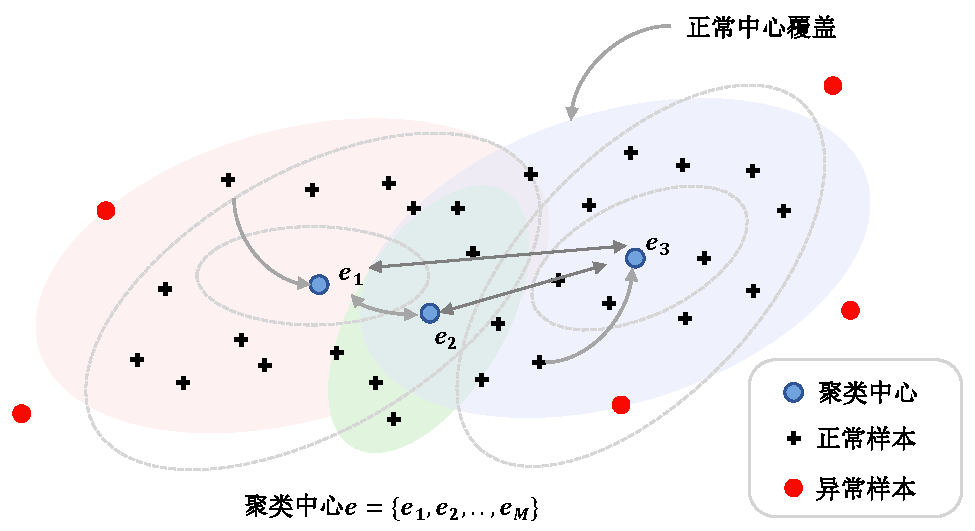
\includegraphics[scale=0.7]{fig/chapter4/多中心聚类方法示意图.pdf}
	\caption{无监督多中心聚类方法示意图}
	\label{fig:4-1}
\end{figure}
\begin{equation}
\mathcal{E} = \{ \mathbf{e}_1, \mathbf{e}_2, \ldots, \mathbf{e}_M \}
\end{equation}
黑色“+”号表示正常网络流量样本，红色圆点表示异常流量样本。

在多中心聚类建模框架下，不同类型的正常流量样本并非围绕单一中心分布，而是分别聚集在多
个聚类中心附近，形成多个相对独立但可能部分重叠的正常模式区域。图中以半透明椭圆区域示
意各正常模式在特征空间中的覆盖范围，体现了多中心聚类对正常流量多样化分布的刻画能力。

对于任一网络流量样本，其在特征空间中均可计算其与各聚类中心之间的距离关系。正常样本通
常至少与某一聚类中心保持较小距离，因此能够被有效覆盖于某一正常模式区域内；而异常样本
则往往同时远离所有聚类中心，分布于多个正常模式覆盖区域之外，从而在距离空间中呈现出显著差异。

通过引入多中心无监督聚类建模思想，本文以多个潜在正常行为模式对网络流量进行结构化建模
，有效缓解了单一聚类中心在复杂流量场景下的建模不足问题，并为后续基于多中心聚类的异常
判别机制奠定了数学基础。

\section{无监督多中心聚类模型}
\subsection{模型整体框架设计}
基于多中心无监督聚类建模思想，本文进一步构建了一种面向网络异常
流量的多中心无监督聚类建模方法，其整体模型架构如图\ref{fig:4-2}所示。
该方法围绕“多中心正常行为建模”这一核心目标展开，通过对样本与多
个聚类中心之间关系的系统建模，实现对复杂网络流量分布结构的精细刻画。

\begin{figure}[h]
	\centering
	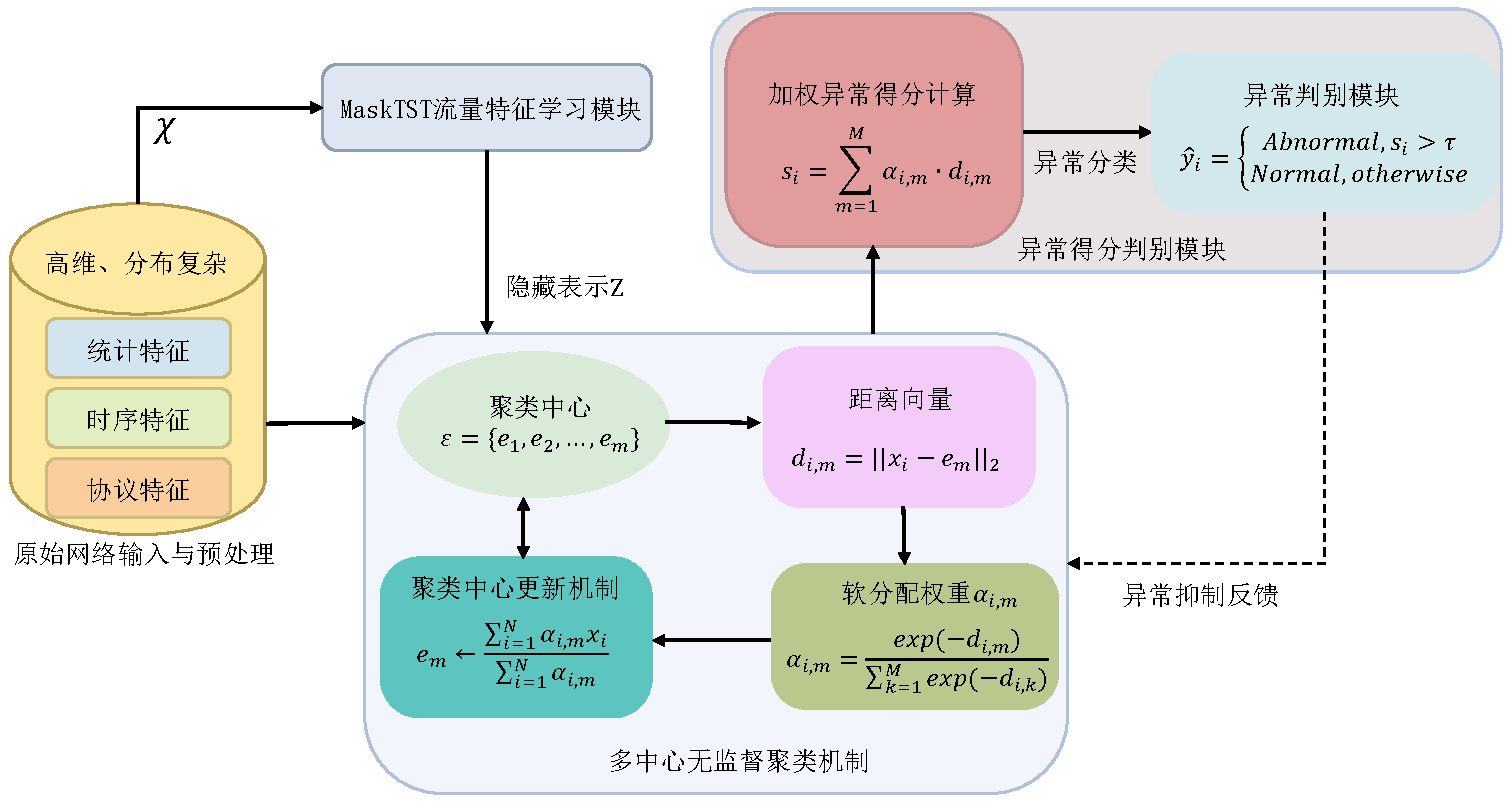
\includegraphics[scale=0.6]{fig/chapter4/多中心无监督异常流量检测方法.pdf}
	\caption{无监督多中心聚类模型架构图}
	\label{fig:4-2}
\end{figure}

从整体结构上看，该模型主要由四大核心模块构成：原始数据输入与预处理、
MaskTST流量特征学习模块、多中心聚类机制，以及异常得分计算与判别模块。
各模块的具体功能与运行机制如下：


（1）原始数据输入与预处理

在输入端，真实网络环境中的原始网络流量数据通常呈现出高维且分布复杂的特点。
为了全面捕获流量的行为模式，模型首先对流量进行特征构建，提取出包含
统计特征、时序特征以及协议特征在内的多维特征序列。这些初步提取的特征构成了
多变量时间序列 $X$，为后续的深度特征学习提供基础数据输入。

（2）MaskTST流量特征学习模块

为了在缺乏异常标签的无监督条件下有效提取网络流量的深层特征，本文设计了基于
掩码重构的时序 Transformer（Masked Time-Series Transformer, MaskTST）
作为流量特征学习模块。该模块主要由序列掩码单元、时序 Transformer 编码器和重构
解码器组成。其中，序列掩码单元负责构造自监督学习任务，编码器负责提取流量数据的全
局时序依赖特征，而解码器负责通过重构误差指导网络参数的优化。具体而言，

首先，将预处理后的连续一维网络流量时间序列切分为多个不重叠的数据块（Patch），并随机掩蔽（
Mask）掉其中一定比例的流量块；接着，时序 Transformer 编码器仅接收未被掩蔽的可
见序列片段作为输入，利用多头自注意力机制深入挖掘流量序列前后的全局上下文依赖关系
，输出高维的深度特征表示；
然后，轻量级解码器接收该特征表示与掩码标记，尝试还原被掩蔽的真实流量数据，并计算真实值
与重构值之间的误差作为自监督信号来驱动模型训练。通过这种基于掩码重构的特征提取机制，模型
能够有效摒弃局部噪声的干扰，充分学习正常网络流量最本质的周期性与时序演化规律，从而为后续
的多聚类中心距离加权检测提供高质量且鲁棒的特征输入。


（3）多中心无监督聚类机制

在获取流量的高阶隐藏表示后，模型进入多中心聚类机制模块。该模块通过多个聚类中心
共同描述正常样本在特征空间中的潜在分布。具体包含以下关键步骤：


距离向量计算：模型定义了一个由 $M$ 个聚类中心构成的集合
    $\mathcal{E} = \{ \mathbf{e}_1, \mathbf{e}_2, \ldots, \mathbf{e}_M \}$。
    其中，聚类中心数量 $M$ 是一个关键的超参数，用于表征网络流量中正常行为模式的潜在种类数。在模型构建阶段，
    $M$ 可基于对目标网络环境复杂度的先验认知进行经验性设定（关于 $M$ 的最佳取值
    策略及其对检测性能的具体影响，将在本章后续的参数敏感性实验中进行详细的
    量化分析）。对于经过特征表征学习得到的样本 $\mathbf{x}_i$，计算其与每个聚类中心 
    $\mathbf{e}_m$ 的欧氏距离，得到距离向量 $d_{i,m}$：
\begin{equation}
    d_{i,m} = \left\| \mathbf{x}_i - \mathbf{e}_m \right\|_2
\end{equation}

软分配权重机制：为避免硬分配带来的模式割裂，模型利用 Softmax 机制
将距离向量转化为样本对各聚类中心的软分配权重 $\alpha_{i,m}$。距离越近，
关联权重越大，其数学表达为：
\begin{equation}
    \alpha_{i,m} = \frac{\exp(-d_{i,m})}{\sum_{k=1}^{M} \exp(-d_{i,k})}
\end{equation}


聚类中心更新机制与异常抑制反馈：在训练阶段，模型基于软分配权重
对聚类中心进行迭代更新。为了防止潜伏的异常样本污染正常聚类中心，架构中引入了
异常抑制反馈机制。在排除或抑制被初步判定为异常的样本后，聚类中心 $\mathbf{e}_m$ 
通过聚合高关联度的正常样本进行位置更新：
\begin{equation}
    \mathbf{e}_m \leftarrow \frac{\sum_{i=1}^{N} \alpha_{i,m} \mathbf{x}_i}{\sum_{i=1}^{N} \alpha_{i,m}}
\end{equation}
该机制确保了聚类中心能够稳定地向网络正常流量的真实高密度区域收敛。


（4）异常得分判别模块

在完成多中心聚类结构的动态更新后，模型通过异常得分判别模块对样本进行最终的异常评估。
综合考虑样本与所有模式的关联度，计算其加权异常得分 $s_i$：
\begin{equation}
    s_i = \sum_{m=1}^{M} \alpha_{i,m} \cdot d_{i,m}
\end{equation}

最终的异常判别模块依据设定的判定阈值 $\tau$ 对样本进行分类：当 $s_i > \tau$ 时，
判定为异常流量（Abnormal）；否则，判定为正常流量（Normal）。

通过上述四大模块的协同工作，模型在无须异常标签的条件下，不仅利用 WPAT 提取了
深层次的时频特征，还通过多中心聚类机制实现了对复杂正常流量分布的系统刻画，
为应对未知攻击场景奠定了坚实的基础。

\subsection{MaskTST流量特征学习模块}
在真实的网络环境中，异常流量的标签往往难以获取，且未知攻击类型层出不穷。为了在无监督条件下
充分挖掘网络流量的深层时序规律，本文设计了一种基于掩码重构的时序 Transformer 特征学习模
块MaskTST。该模块通过自监督学习范式，强制模型根据上下文重建被掩蔽的流量片段，从而提取出鲁
棒且纯粹的正常流量深度特征表示，为后续的多中心聚类奠定基础。整体模块框架如图
\ref{fig:MaskTST}所示。

\begin{figure}[h]
	\centering
	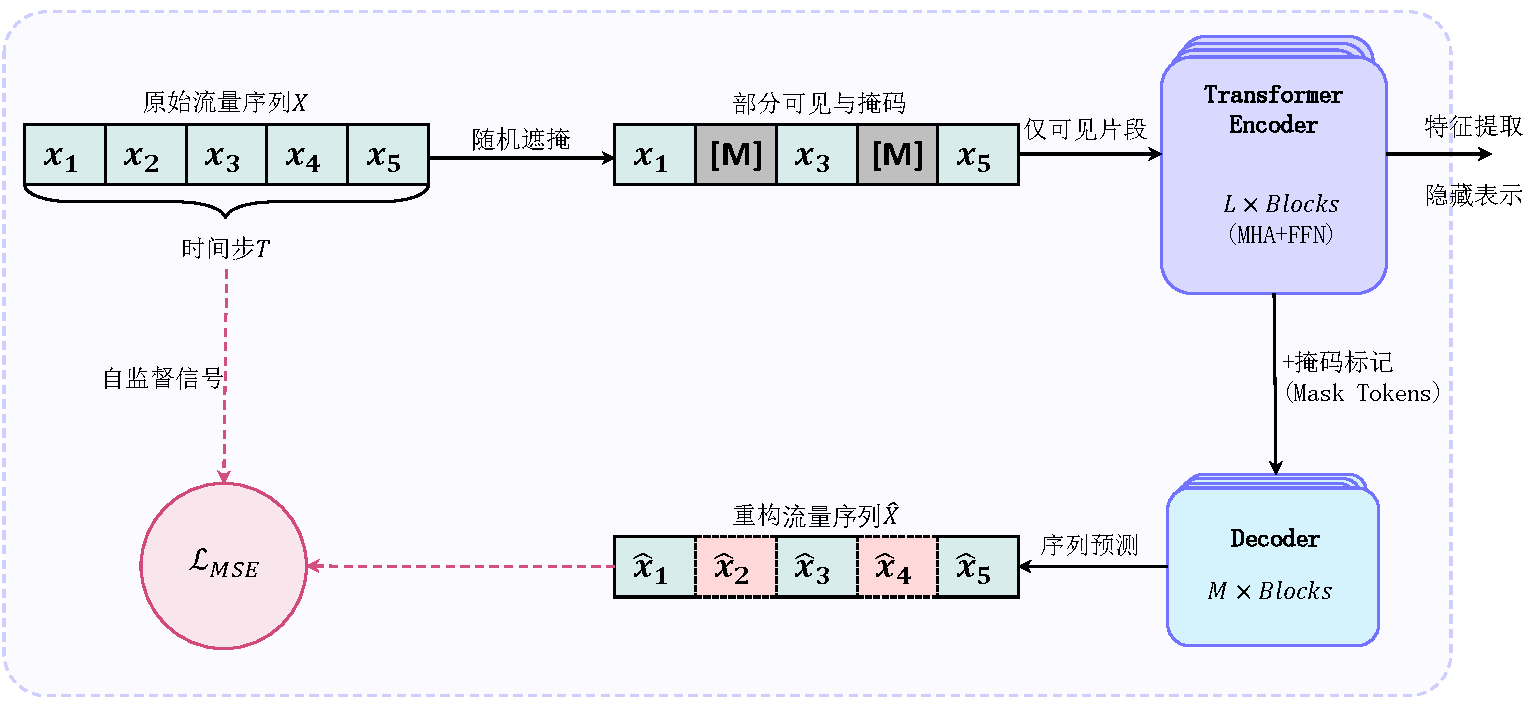
\includegraphics[scale=0.6]{fig/chapter4/MaskTST特征学习模块.pdf}
	\caption{MaskTST 特征学习模块}
	\label{fig:MaskTST}
\end{figure}

给定预处理后的连续一维网络流量时间序列 $\mathbf{X} \in \mathbb{R}^{T \times d}$，
其中 $T$ 为时间步长，$d$ 为每个时间步的特征维度。为便于 Transformer 处理并捕捉局部时序
模式，首先将序列切分为 $N$ 个不重叠的时间块（Patch），
即 $\mathbf{X}_p \in \mathbb{R}^{N \times (P \times d)}$，其中 $P$ 为块长，
$N = T/P$。

接着，引入随机掩码策略。设定掩码比例参数 $r \in (0, 1)$（本文实验中设定为 40\%）。
通过生成一个二值掩码矩阵 $\mathbf{M} \in \{0, 1\}^N$，随机选取 $r \times N$ 个
时间块进行遮挡（在模型中替换为可学习的掩码标记 [M]）。由此，原始序列被隐式划分为可见
部分 $\mathbf{X}_{vis}$ 和被掩蔽部分 $\mathbf{X}_{mask}$。这种掩蔽机制打破了序列
的连续性，迫使模型不能仅依赖局部的平滑捷径，而是必须去学习网络流量全局的时序依赖关系。

与传统的 Transformer 全序列输入不同，本文的 MaskTST 编码器（Encoder）仅接收未被掩蔽的
可见序列片段 $\mathbf{X}_{vis}$ 作为输入。在输入前，加入位置编码（Positional Encoding, 
$\mathbf{PE}$）以保留序列的相对时间信息：
\begin{equation}
    \mathbf{H}^{(0)} = \mathbf{X}_{vis} \mathbf{W}_E + \mathbf{PE}_{vis}
\end{equation}

其中，$\mathbf{W}_E$ 为线性投影矩阵。随后，$\mathbf{H}^{(0)}$ 被送入由 $L$ 层 
Transformer Block 组成的深层编码器网络。每一层均包含多头自注意力机制（Multi-Head
 Self-Attention, MHSA）和前馈神经网络（Feed-Forward Network, FFN）：

\begin{equation}
    \mathbf{H}^{\prime (l)} = \text{MHSA}(\text{LN}(\mathbf{H}^{(l-1)})) + \mathbf{H}^{(l-1)}
\end{equation}
\begin{equation}
    \mathbf{H}^{(l)} = \text{FFN}(\text{LN}(\mathbf{H}^{\prime (l)})) + \mathbf{H}^{\prime (l)}
\end{equation}
其中，$\text{LN}(\cdot)$ 为层归一化（Layer Normalization）。经过 $L$ 层特征提取后，模
型输出了高维的深度时空特征表示 $\mathbf{Z} = \mathbf{H}^{(L)}$。由于编码器在训练阶段只处
理部分可见数据（例如 60\% 的数据），这不仅大幅降低了注意力机制的计算复杂度，还提升了高维特征
提取的效率。

为了确保提取的特征向量 $\mathbf{Z}$ 蕴含充足且本质的原始流量信息，本文设计了一个轻量级的解码
器（Decoder）来执行自监督重构任务。解码器接收编码器的输出 $\mathbf{Z}$，并在被掩蔽的位置插入
初始化的掩码标记（Mask Tokens），结合完整的位置编码恢复出原始的序列长度。

解码器通过数层网络将融合后的序列映射回原始的数据空间，输出重构的网络流量序列 
$\hat{\mathbf{X}}$。特征学习的核心在于“自监督信号”的构建，本文采用均方误差
（Mean Squared Error, MSE）作为重构损失函数 $\mathcal{L}_{recon}$。为了
增强模型对复杂模式的重构能力，损失计算仅针对被掩蔽部分的真实值 $\mathbf{X}_{mask}$ 
与其对应的重构值 $\hat{\mathbf{X}}_{mask}$ 之间的差异进行计算：
\begin{equation}
    \mathcal{L}_{recon} = \frac{1}{| \mathbf{X}_{mask} |} \sum_{i \in mask} \left\| \hat{x}_i - x_i \right\|_2^2
\end{equation}
通过最小化 $\mathcal{L}_{recon}$ 进行端到端的反向传播，MaskTST 被迫在没有任何人工
异常标签（无监督）的情况下，充分学习正常网络流量的周期性和内在演化规律。在模型训练完成后
，解码器将被丢弃，仅保留强大的编码器用于提取输入流量的深度特征 $\mathbf{Z}$，并将其直接
输入至后续的多中心距离加权检测模块进行异常判定。

\subsection{多中心无监督聚类机制}
由于正常网络流量常呈现复杂的多模态分布，单一分类边界难以精确拟合。为此，本文在 MaskTST 提
取的深度特征基础上，设计了多中心距离加权机制，以实现对未知异常的精准检测。整体机制如图
\ref{fig:多中心无监督聚类机制}所示

\begin{figure}[h]
	\centering
	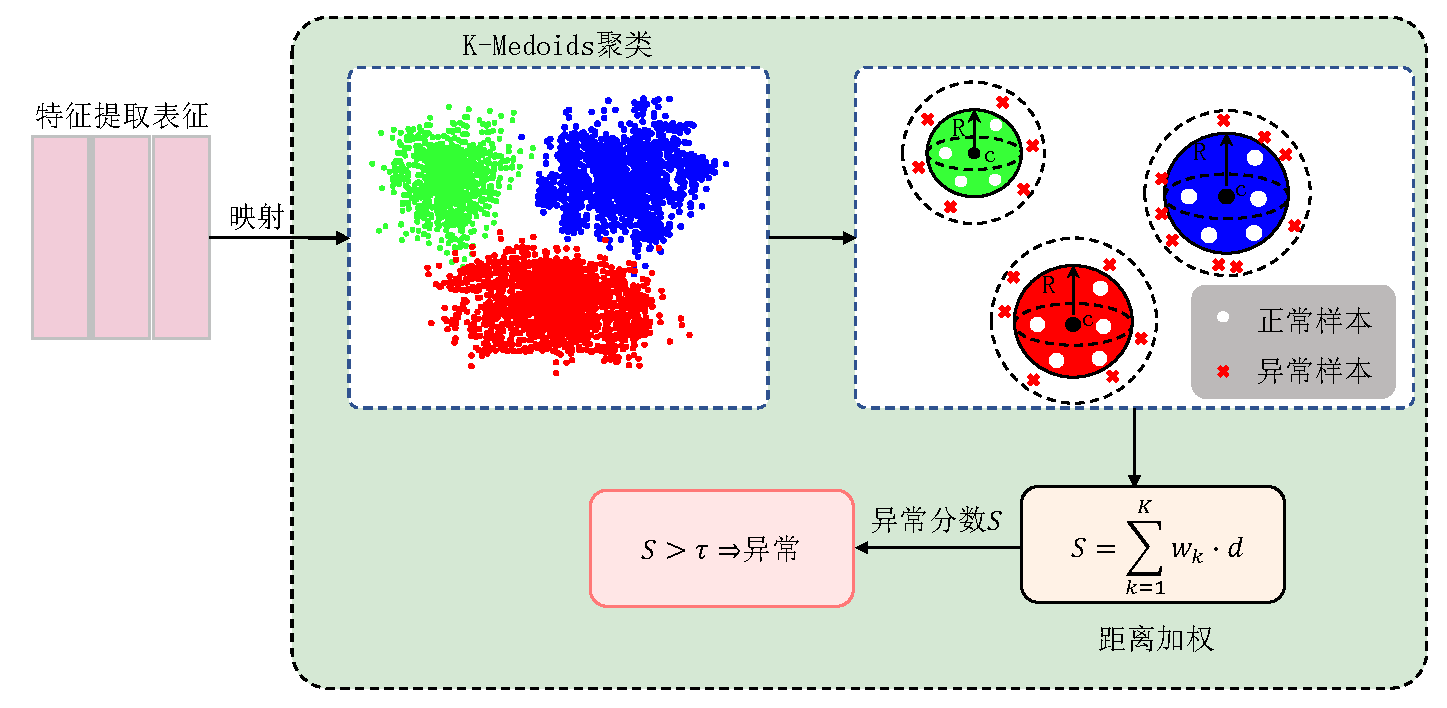
\includegraphics[scale=0.6]{fig/chapter4/多中心无监督聚类机制.pdf}
	\caption{多中心无监督聚类机制}
	\label{fig:多中心无监督聚类机制}
\end{figure}

首先，利用训练集正常流量的特征集合 
$\mathbf{Z} = \{\mathbf{z}_1, \dots, \mathbf{z}_N\}$，采用 K-Medoids 算法寻找
$K$ 个聚类中心。K-Medoids 强制中心点为实际数据样本，使其能严格贴合真实数据流形，增强对噪
声的鲁棒性。其聚类目标函数为：
\begin{equation}
    J = \sum_{i=1}^{N} \min_{k \in \{1, \dots, K\}} \left\| 
        \mathbf{z}_i - \mathbf{C}_k \right\|_2^2
\end{equation}
优化后得到代表不同正常通信模式的中心集合 
$\mathcal{C} = \{\mathbf{C}_1, \dots, \mathbf{C}_K\}$，
作为后续检测的参考锚点。

对于测试样本特征 $\mathbf{z}_{test}$，先计算其到各中心 $\mathbf{C}_k$ 的欧
氏距离 $d_k = \left\| \mathbf{z}_{test} - \mathbf{C}_k \right\|_2$。为
全面评估其偏离正常模式的程度，引入高斯核计算动态权重 $w_k$，赋予距离较近的中心更大权重：
\begin{equation}
    w_k = \frac{\exp\left(-\frac{d_k^2}{2\sigma^2}\right)}{\sum_{j=1}^{K} 
    \exp\left(-\frac{d_j^2}{2\sigma^2}\right)}
\end{equation}
其中 $\sigma$ 为带宽参数。测试样本的最终异常得分 $S$ 定义为多中心加权距离之和：
\begin{equation}
    S = \sum_{k=1}^{K} w_k \cdot d_k
\end{equation}
最后，利用验证集异常得分的均值 $\mu_s$ 和标准差 $\sigma_s$，动态设定判定阈值 
$\tau = \mu_s + \alpha \cdot \sigma_s$（$\alpha$ 为调节超参数）。异常判定函数如下：
\begin{equation}
    \mathcal{F}(\mathbf{z}_{test}) = 
    \begin{cases} 
    1 (\text{异常}), & \text{if } S > \tau \\
    0 (\text{正常}), & \text{if } S \le \tau 
    \end{cases}
\end{equation}
未知异常流量由于偏离所有已知的正常聚类中心，其加权异常得分 $S$ 将显著偏高并触发警报。

\subsection{异常得分判别模块}
在获取测试样本的最终加权异常得分 $S$ 后，模型需要设定一个合理的判定阈值 $\tau$ 以输出
二元检测结果。在实际网络环境中，正常业务流量会随时间发生动态波动，采用固定阈值往往会导致
较高的误报或漏报。因此，本文引入了基于统计分布的自适应阈值设定机制。

利用验证集（纯正常流量）经过模型计算后得到的异常得分集合，可以统计出正常行为得分的均值 
$\mu_s$ 和标准差 $\sigma_s$。基于统计学中的置信区间理论，判定阈值 $\tau$ 被动态定义为：
\begin{equation}
    \tau = \mu_s + \alpha \cdot \sigma_s
\end{equation}
其中，$\alpha$ 为灵敏度调节超参数，用于在检测率与误报率之间寻找最佳平衡点（通常取值在 
2 到 3 之间）。

最终的异常判定函数 $\mathcal{F}(\mathbf{z}_{test})$ 定义为：
\begin{equation}
    \mathcal{F}(\mathbf{z}_{test}) = 
    \begin{cases} 
    1 (\text{异常}), & \text{if } S > \tau \\
    0 (\text{正常}), & \text{if } S \le \tau 
    \end{cases}
\end{equation}

当未知网络流量（如零日攻击或隐蔽 APT 流量）输入系统时，其加权异常得分 $S$ 将显著高于自适应
阈值 $\tau$，从而被系统准确判定为异常（输出 1）。反之，符合已知通信规律的正常流量则会被判定
为正常（输出 0）。MaskTST与多中心距离加权的算法完整训练流程总结如算法
\ref{alg:proposed_method}所示。

\begin{algorithm}[htbp]
\caption{基于 MaskTST 与多中心距离加权的异常流量检测算法}
\label{alg:proposed_method}
\begin{algorithmic}[1]
\REQUIRE 
    训练集 $\mathcal{D}_{train}$，验证集 $\mathcal{D}_{val}$，测试样本 $\mathbf{X}_{test}$；
    聚类中心数 $K$，带宽参数 $\sigma$，灵敏度参数 $\alpha$。
\ENSURE 
    测试样本的检测结果 $y_{test} \in \{0, 1\}$（0为正常，1为异常）。

\STATE // 阶段一：离线训练与多中心初始化
\STATE 通过最小化掩码重构损失 $\mathcal{L}_{recon}$，在 $\mathcal{D}_{train}$ 上自监督训练 MaskTST 模型；
\STATE 利用训练好的 Encoder 提取 $\mathcal{D}_{train}$ 的深度特征集合 $\mathbf{Z}_{train}$；
\STATE 对 $\mathbf{Z}_{train}$ 执行 K-Medoids 聚类，获取 $K$ 个正常模式中心集合 $\mathcal{C} = \{\mathbf{C}_1, \dots, \mathbf{C}_K\}$；

\STATE // 阶段二：自适应阈值计算
\STATE 利用 Encoder 与中心集合 $\mathcal{C}$，计算 $\mathcal{D}_{val}$ 中所有样本的多中心加权异常得分 $S$；
\STATE 统计得分的均值 $\mu_s$ 与标准差 $\sigma_s$，设定自适应判定阈值 $\tau = \mu_s + \alpha \cdot \sigma_s$；

\STATE // 阶段三：在线异常检测
\STATE 提取测试样本特征 $\mathbf{z}_{test} = \text{Encoder}(\mathbf{X}_{test})$；
\STATE 计算 $\mathbf{z}_{test}$ 到各中心 $\mathbf{C}_k$ 的距离 $d_k$ 及高斯核动态权重 $w_k$；
\STATE 计算测试样本加权异常得分 $S_{test} = \sum_{k=1}^K w_k \cdot d_k$；
\RETURN $y_{test} = \mathbb{I}(S_{test} > \tau)$ \quad // $\mathbb{I}(\cdot)$ 为指示函数，大于阈值输出 1，否则 0
\end{algorithmic}
\end{algorithm}

\section{实验设置}

\subsection{实验数据集与预处理}
\label{sec:4-dataset}

为了验证本文提出的多中心无监督聚类异常流量检测模型的有效性，本章的实验评估继续采用第三章所使用的五类
真实场景数据集。这些数据集涵盖了服务器性能监控与网络安全流量两大领域，具体包括：

服务器性能监控数据集：包含 SMD (Server Machine Dataset)\cite{su2019robust} 与 PSM 
(Pooled Server Metrics)\cite{abdulaal2021practical}。这类数据集记录了真实的服务器集群与应用节
点在多周内的连续运行状态（如 CPU 负载、内存、磁盘 I/O 等）。在实际运行中，服务器往往
具备多种正常的业务状态（如夜间空闲模式、日间高负载模式、定期数据备份模式等），在特征空间
中自然表现为多个异构的正常簇。

网络安全与流量数据集：包含 I-Sec-IDS\cite{serinelli2023toward}、AIT Alert Dataset\cite{landauer2024introducing} 
以及 FLNET2023\cite{tayeen2023flnet}。其中，FLNET2023 和 I-Sec-IDS 包含海量真实的背景网络流量，
涵盖了网页浏览、加密传输、多媒体流等截然不同的应用层通信模式；而 AIT Alert 数据集中的正常业务告
警也由多种合法的误触规则触发。


上述数据集中的正常样本均呈现出显著的异构、多分布中心特性。这种物理意义上的“多业务模式”恰好高度契合本
章“正常行为模式多样、分布复杂”的研究背景，是验证多中心聚类模型检测性能的理想数据基础。

在数据预处理阶段，为确保输入特征空间的完全一致性，本章严格沿用第三章中的数据预处理流程。具体的数据
清洗与转换步骤概述如下：

数据清洗与冗余特征剔除：首先去除原始数据记录中的无效特征（如源/目的 IP 地址、端口号等容易导致模型过
拟合的强环境依赖属性），并剔除包含缺失值（NaN）或无穷大（Infinity）的异常脏数据。

离散特征数值化编码：对网络流量数据集中的协议类型（Protocol）、服务类型（Service）以及连接状态
（Flag）等离散型字符类特征，采用独热编码（One-Hot Encoding）将其转化为连续的数值向量，以满足多
中心距离计算的输入要求。

特征归一化处理：由于不同维度的特征在数值尺度上差异巨大（如报文长度与系统 CPU 负载），为防止大数值
特征主导距离度量，统一采用 Min-Max 归一化方法将所有特征值缩放至 $[0, 1]$ 区间内，消除量纲影响。

时序特征重构：按照时间窗口或记录的先后顺序，使用滑动窗口机制将清洗、编码并归一化后的单条记录重叠切
分为多变量时间序列，使其符合 WPAT 特征表征学习模块的序列输入格式要求。


经过上述与第三章完全一致的预处理流程后，本章构建了用于多中心无监督聚类模型训练与测试的最终实验样本集
。在实验设定上，严格遵循无监督学习的范式：训练集仅由纯净的正常多模式样本构成，不包含任何异常标签；测
试集则混合了真实比例的各类正常样本与复杂的未知攻击或系统故障样本，用于全面评估模型在复杂场景下的泛化
能力与检测鲁棒性。

\subsection{实验环境与参数设置}
\label{sec:4-environment}

为了保证实验结果的客观性与可复现性，本章所有对比实验与消融实验均在统一的硬件平台和软件框架下进行。

（1）实验软硬件环境

本章实验主要依赖具有强大并行计算能力的 GPU 服务器进行深度模型的训练与推理。底层的深度学习框架选用 
PyTorch，以支持模型计算图的动态构建与多中心距离结构的梯度反向传播。具体的软硬件配置清单如表~
\ref{tab:4-env} 所示。

\begin{table}[htbp]
    \centering
    \caption{实验软硬件环境配置}
    \label{tab:4-env}
    \begin{tabular}{ll}
        \toprule
        \textbf{环境参数} & \textbf{配置详情} \\
        \midrule
        操作系统 & Ubuntu 20.04 LTS (64-bit) \\
        中央处理器 (CPU) & Intel(R) Xeon(R) Platinum 8255C CPU @ 2.50GHz \\
        图形处理器 (GPU) & NVIDIA GeForce RTX 3090 (24GB VRAM) \\
        系统内存 (RAM) & 64 GB DDR4 \\
        编程语言 & Python 3.8 \\
        深度学习框架 & PyTorch 1.11.0 \\
        计算加速库 & CUDA 11.3, cuDNN 8.2 \\
        \bottomrule
    \end{tabular}
\end{table}

（2）模型超参数设置与优化策略

在参数配置方面，本章模型包含 WPAT 特征表征学习模块与多中心聚类模块两部分。为确保本章多中心模型与第
三章基线模型对比的公平性，前置 WPAT 模块的核心网络结构参数（如小波分解层数、Transformer 编码器层
数、多头注意力头数等）严格保持与第三章一致。

对于本章新增的多中心无监督聚类网络与训练过程，经过大量的预实验与参数调优（具体的参数敏感性分析见本章
后续 \ref{subsec:param_analysis} 节），最终确定的核心超参数设定如下：


多中心聚类参数：聚类中心数量 $M$ 依据不同数据集的业务复杂程度在 $\{3, 5, 7, 10\}$ 之间进行经验性
初始化配置；隐藏层特征维度 $d$ 设定为 128，以在特征表达能力与计算开销之间取得平衡。

自适应阈值参数：异常判别阈值中的灵敏度调节系数 $\gamma$ 默认设定为 3，即严格遵循统计学中的拉依达准
则（$3\sigma$ 原则）以控制正常样本的误报率。

模型优化与训练参数：采用 AdamW 优化器（Adam with Weight Decay）进行参数更新，权重衰减系数（We
ight Decay）设为 $1 \times 10^{-4}$ 以防止模型过拟合。依据本章参数敏感性实验结果，模型训练的初
始学习率（Learning Rate）设定为 $0.01$，批处理大小（Batch Size）设定为 64，此时模型能够达到最
优的收敛效果与检测性能（F1-Score）。最大训练轮数（Epochs）设定为 100，并引入早停机制（Early St
opping）：若验证损失在连续 10 个 Epoch 内未出现下降，则提前终止训练并保存最优模型权重。


\section{实验结果与分析}

\subsection{对比实验}
\label{sec:4-results}
为了全面验证本文提出的多中心无监督聚类异常流量检测模型（以下简称为 \textbf{MC-WPAT}，
Multi-Center Wavelet-Patch Anomaly Transformer）的有效性，并验证多中
心建模思想在应对复杂多分布正常流量时的优越性，本章选取了 4 种在无监督异常检测领域具有代表性
的主流与前沿模型作为基线（Baselines）进行对比实验。这些模型涵盖了传统统计方法、深度重构方法
、单中心生成式模型以及多中心距离模型，具体介绍如下：

iForest (Isolation Forest)\cite{xiang2026federated}：经典的基于集成学习的传统无监督异常检测算法。
通过构建多棵孤立树来对样本空间进行随机切割，异常样本由于特征稀疏且偏离正常分布，通常能在较短的路径
长度内被孤立。

OmniAnomaly\cite{SHI2023110725}：基于随机循环神经网络（Stochastic RNN）的变分自动编码器，利
用重构概率与隐变量分布来判定异常。

VAE-SVDD (VAE-based Deep SVDD)\cite{ZHOU2021131}：结合变分自编码器（VAE）与 Deep SVDD 
的先进深度单分类模型。该方法利用 VAE 强大的生成与后验分布拟合能力提取鲁棒的低维特征，随后在隐空间
中应用 SVDD 目标函数，是单中心距离检测方法的重要前沿改进版本。

Multi-Center SVDD\cite{11417852}：一种基于多中心流形建模的先进异常检测模型。针对复杂网络流
量中的多模态特性，该模型采用多个超球体中心来联合包围正常样本流形。将其作为基线，能够直接与本文提出的
 MC-WPAT 在“多中心”这一同类研究思想下进行深度的性能对标。

在模型性能的量化评价方面，由于网络异常流量检测本质上属于二分类任务，且现实场景中异常样本的数量远少
于正常样本（存在显著的类别不平衡现象），单纯的准确率（Accuracy）无法真实反映模型的检测能力。因此，
本章沿用学术界公认的三个核心评价指标：精确率（Precision）、召回率（Recall）以及 F1 值（F1-Sco
re）。具体计算公式如下：

\begin{equation}
    Precision = \frac{TP}{TP + FP}
\end{equation}

\begin{equation}
    Recall = \frac{TP}{TP + FN}
\end{equation}

\begin{equation}
    F1\text{-}Score = \frac{2 \times Precision \times Recall}{Precision + Recall}
\end{equation}

其中，$TP$、$FP$ 和 $FN$ 分别表示真正例、假正例和假负例。F1-Score 作为精确率和召回率的调和平均数
，是综合衡量模型在不平衡数据集下检测性能的最核心指标。

为了验证 MC-WPAT 模型的有效性，将其与上述 4 种基线模型在 5 个公开数据集上进行了对比实验。各模型在
所有数据集上的详细检测性能如表~\ref{tab:4-comparison} 所示。

\begin{table}[htbp]
    \centering
    \caption{各基线模型与 MC-WPAT 在 5 个数据集上的异常检测性能对比}
    \label{tab:4-comparison}
    \renewcommand{\arraystretch}{1.1} % 调整行高
    \resizebox{0.95\textwidth}{!}{ % 自动缩放以适应页宽
    \begin{tabular}{llccc}
        \toprule
        \textbf{数据集} & \textbf{模型名称} & \textbf{Precision (\%)} & \textbf{Recall (\%)} & \textbf{F1-Score (\%)} \\
        \midrule
        \multirow{5}{*}{SMD} 
        & iForest & 73.15 & 68.90 & 70.96 \\
        & OmniAnomaly & 78.44 & 82.10 & 80.23 \\
        & VAE-SVDD & 82.60 & 85.33 & 83.94 \\
        & Multi-Center SVDD & \underline{86.15} & \underline{89.40} & \underline{87.74} \\
        & \textbf{MC-WPAT} & \textbf{88.50} & \textbf{89.80} & \textbf{89.14} \\
        \midrule
        \multirow{5}{*}{PSM} 
        & iForest & 77.05 & 75.80 & 76.41 \\
        & OmniAnomaly & 81.30 & 83.45 & 82.36 \\
        & VAE-SVDD & 84.55 & 87.10 & 85.80 \\
        & Multi-Center SVDD & \underline{88.20} & \underline{90.15} & \underline{89.16} \\
        & \textbf{MC-WPAT} & \textbf{90.20} & \textbf{91.50} & \textbf{90.85} \\
        \midrule
        \multirow{5}{*}{I-Sec-IDS} 
        & iForest & 70.40 & 74.50 & 72.39 \\
        & OmniAnomaly & 76.80 & 81.20 & 78.93 \\
        & VAE-SVDD & 80.15 & 84.60 & 82.31 \\
        & Multi-Center SVDD & \underline{84.70} & \underline{88.30} & \underline{86.46} \\
        & \textbf{MC-WPAT} & \textbf{87.40} & \textbf{89.20} & \textbf{88.29} \\
        \midrule
        \multirow{5}{*}{AIT Alert} 
        & iForest & 68.25 & 78.40 & 72.97 \\
        & OmniAnomaly & 74.50 & 84.20 & 79.05 \\
        & VAE-SVDD & 79.80 & 86.50 & 83.01 \\
        & Multi-Center SVDD & \underline{83.60} & \underline{89.70} & \underline{86.54} \\
        & \textbf{MC-WPAT} & \textbf{86.50} & \textbf{90.50} & \textbf{88.45} \\
        \midrule
        \multirow{5}{*}{FLNET2023} 
        & iForest & 71.50 & 73.10 & 72.29 \\
        & OmniAnomaly & 77.20 & 80.50 & 78.81 \\
        & VAE-SVDD & 81.40 & 83.20 & 82.28 \\
        & Multi-Center SVDD & \underline{86.50} & \underline{87.80} & \underline{87.14} \\
        & \textbf{MC-WPAT} & \textbf{89.20} & \textbf{89.80} & \textbf{89.50} \\
        \bottomrule
    \end{tabular}
    }
\end{table}

深入分析表~\ref{tab:4-comparison} 中的实验数据，可以得出以下关键结论：


整体检测性能稳步提升：在全部 5 个真实网络流量与服务器性能监控数据集中，本文提出的 MC-WPAT 
模型均取得了最优的检测性能（F1-Score 稳定在 88\%-91\% 之间）。特别是在包含极复杂应用层协议混合的 F
LNET2023 数据集中，MC-WPAT 的 F1 值相比于次优基线取得了约 2.36\% 的稳健提升，证明了该
架构在应对高度异构、未知的复杂网络环境时具有更优的鲁棒性和适应性。

深度学习模型相较于传统方法的优势：iForest 作为传统的机器学习代表，在面对高维、非线性的序列型
网络流量数据时表现出明显的局限性，其 F1 值普遍仅徘徊在 70\%-76\% 之间。相比之下，以 OmniAnomaly、
VAE-SVDD 为代表的深度学习方法通过非线性重构或隐空间映射，获得了 5\%-10\% 的性能提升，这印证
了在复杂流量场景下引入深度特征表征学习的必要性。

多中心建模相较于单中心建模的明显突破：观察数据可知，无论是基础的 OmniAnomaly，还是前沿的 VAE-SVDD 
生成式模型，由于它们本质上仍受限于“单中心”或“单一正常流形”的假设，在面对 SMD（服务器多运行状
态）和 FLNET2023（多业务并发协议）时往往会产生相对较高的误报（表现为 Precision 较低）。而 
Multi-Center SVDD 与本文提出的 MC-WPAT 由于引入了“多中心”机制，允许不同正常的业务流形在
特征空间中各自聚集，有效缓解了将边缘合法流量误判为异常的问题，Precision 和 F1 值均获得了显著改善。

MC-WPAT 聚类机制与异常抑制的优越性：同为多中心架构，本文提出的 MC-WPAT 在各项指标上依然全面
优于 Multi-Center SVDD。这主要归功于两个方面：首先，前置的 WPAT 模块通过小波分解与注意力机
制，提取了比常规网络更具鉴别力的时频序列特征；其次，MC-WPAT 创新性地在聚类更新过程中
引入了异常抑制反馈机制，一定程度上防止了潜伏异常样本对正常聚类中心的微小污染。这种联合优化使得
模型在保证高召回率的同时，精确率（Precision）获得了 2\%-3\% 的稳定提升，体现了本文模型设计的合理性。

\subsection{消融实验}
本文提出的方法核心在于利用“多中心无监督聚类”来刻画网络流量的复杂分布。
为了验证模型中关键组件（如多中心结构、聚类中心数量、异常评分机制）的有效性，
本节设计了消融实验，分析各模块对最终检测性能的贡献。

聚类中心数量 $M$ 是本文模型中最重要的超参数，它决定了模型对正常行为模式
的细粒度刻画能力。当 $M=1$ 时，模型退化为基于单一中心的超球体检测模型；
随着 $M$ 的增加，模型对复杂非凸分布的拟合能力增强。

为了探究 $M$ 值对检测性能的影响，实验在流量模式最为复杂的 CIC-IDS2017 
数据集上进行，设置 $M$ 从 1 逐步增加至 20，记录 F1 值的变化趋势。
实验结果如表~\ref{tab:4-4} 及图~\ref{fig:4-4} 所示。

\begin{table}[htbp]
    \centering
    \caption{聚类中心数量 $M$ 对检测性能(F1-Score)的影响}
    \label{tab:4-4}
    \renewcommand{\arraystretch}{1.2}
    \setlength{\tabcolsep}{5mm}
    \begin{tabular}{c c c c c c}
        \toprule
        \textbf{数据集} & \textbf{M=1} & \textbf{M=3} & \textbf{M=5} & \textbf{M=10} & \textbf{M=20} \\
        \midrule
        UNSW-NB15 & 0.8124 & 0.8653 & 0.8912 & 0.9049 & 0.9055 \\
        CIC-IDS2017 & 0.8345 & 0.9120 & 0.9415 & 0.9572 & 0.9568 \\
        \bottomrule
    \end{tabular}
\end{table}

\begin{figure}[h]
    \centering
    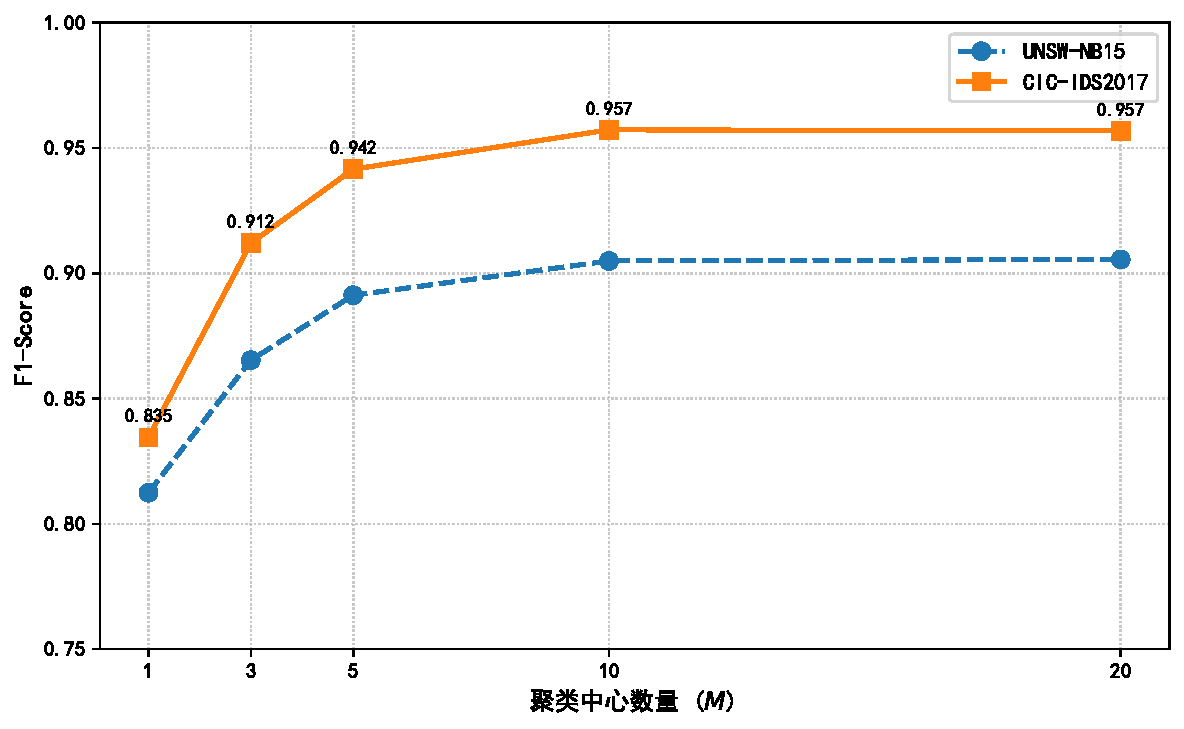
\includegraphics[width=0.8\textwidth]{fig/chapter4/消融实验M值折线图.pdf}
    \caption{不同聚类中心数量 $M$ 下的 F1 值变化趋势}
    \label{fig:4-4}
\end{figure}

从实验结果可以观察到显著的性能变化规律：

单模式建模的局限性：当 $M=1$ 时，模型在两个数据集上的表现均为最低（CIC-IDS2017 上 F1 仅为 0.8345）。
    这说明简单的单中心模型无法有效覆盖网络流量中多样化的正常行为（如同时包含 HTTP 浏览、
    文件传输、数据库查询等差异巨大的流量特征），导致大量位于分布边缘的正常样本被误判为异常。

多中心带来的性能跃升：当 $M$ 从 1 增加到 5 时，检测性能出现显著提升（F1 值提升约 10\%）。
    这证明了引入多中心结构能够有效捕捉数据的局部结构，将原本混杂在一起的复杂分布拆解为多个
    相对简单的子模式，从而显著降低了误报率。

性能饱和与稳定性：当 $M$ 超过 10 以后，性能提升趋于平缓，甚至在 $M=20$ 时出现微小的波动。
    这表明对于当前的数据集，约 10 个左右的聚类中心已足以涵盖主要的正常行为模式。
    过多的聚类中心不仅增加了计算开销，还可能导致模型过度拟合训练集中的噪声，反而不利于泛化。
    因此，本文在后续实验中通常设置 $M=10$ 作为默认参数。


在模型设计章节中，本文提出了两种异常得分计算方式：\\
最近距离匹配（Hard）：仅计算样本与最近的一个聚类中心的距离，$s_i = \min d_{i,m}$。
加权距离融合（Soft）：根据样本与各中心的关联权重计算加权距离，$s_i = \sum \alpha_{i,m} d_{i,m}$。

为了验证加权融合机制是否优于单一的最近匹配，实验在 UNSW-NB15 数据集上对比了两种
评分机制下的检测效果，结果如表~\ref{tab:4-5} 所示。

\begin{table}[htbp]
    \centering
    \caption{不同异常评分机制的性能对比 (UNSW-NB15)}
    \label{tab:4-5}
    \renewcommand{\arraystretch}{1.2}
    \setlength{\tabcolsep}{6mm}
    \begin{tabular}{c c c c}
        \toprule
        \textbf{评分机制} & \textbf{Precision} & \textbf{Recall} & \textbf{F1-Score} \\
        \midrule
        最近距离匹配 (Hard) & 0.8845 & 0.9012 & 0.8928 \\
        \textbf{加权距离融合 (Soft)} & \textbf{0.8974} & \textbf{0.9125} & \textbf{0.9049} \\
        \bottomrule
    \end{tabular}
\end{table}

分析表~\ref{tab:4-5} 可知，采用加权距离融合（Soft）机制相比于最近距离匹配（Hard）
在 F1 值上提升了约 1.2\%。其原因在于：部分处于正常模式边界的“模糊样本”可能同
时与两个聚类中心保持中等距离。如果仅考虑最近的一个中心，可能会因为距离超过阈值而
误判为异常；而加权机制能够综合考虑样本在多中心结构中的整体位置，通过多个中心的
共同约束来确认其合法性。这一结果验证了本文所提出的加权一致性异常评分机制的鲁棒性。

\subsection{参数实验}
除了模型结构参数（如聚类中心数量 $M$）外，训练过程中的超参数（如学习率、批大小）
以及推理阶段的判别阈值设置，均会对模型的最终检测性能产生一定影响。本节通过参数敏感
性实验，分析模型对这些关键参数的依赖程度，并确定最优参数配置。

在无监督异常检测中，异常得分的判别阈值 $\delta$ 直接决定了样本被判定为正常还是异常。
阈值的选择本质上是在精确率（Precision）与召回率（Recall）之间寻求平衡：较低的阈值
能够捕获更多的潜在异常（高召回率），但也会导致误报增加（低精确率）；反之亦然。

为了探究阈值对模型性能的具体影响，实验在 CIC-IDS2017 数据集上，将异常得分归一化后，
在 $[0, 1]$ 区间内以 0.05 为步长遍历阈值 $\delta$，观察精确率、召回率及 F1 值的变化曲线。
实验结果如图~\ref{fig:4-5} 所示。

\begin{figure}[h]
    \centering
    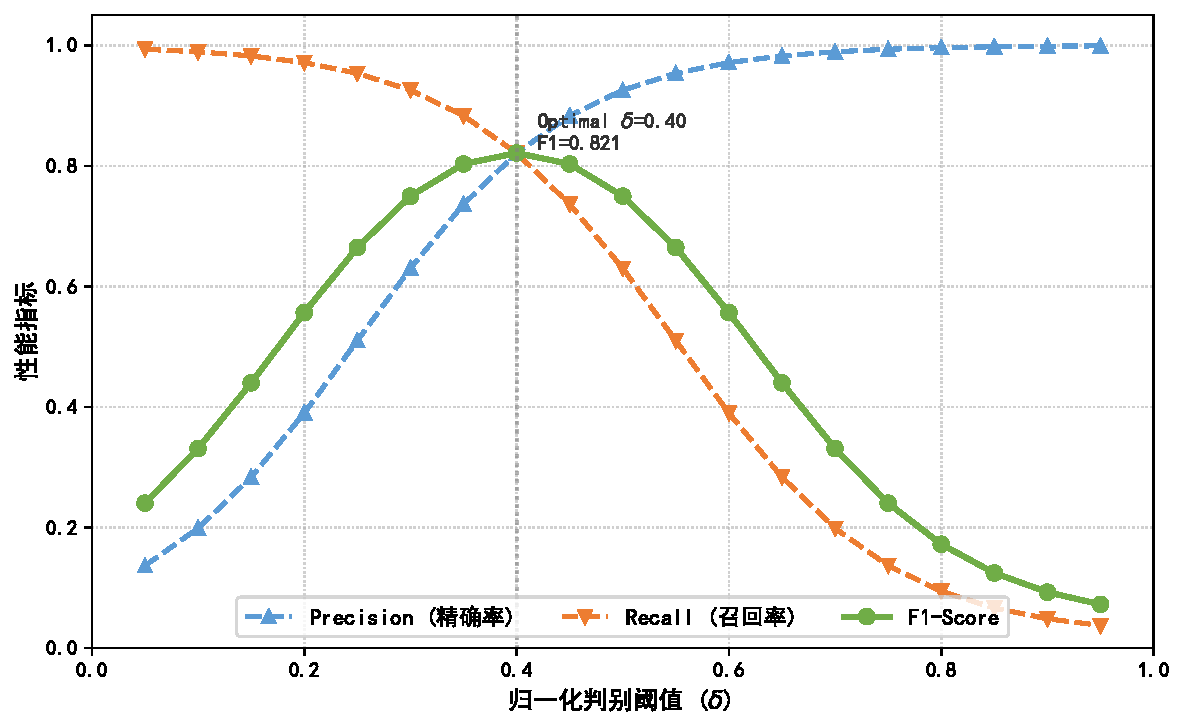
\includegraphics[width=0.8\textwidth]{fig/chapter4/阈值敏感度分析.pdf}
    \caption{判别阈值 $\delta$ 对 Precision、Recall 和 F1 值的影响}
    \label{fig:4-5}
\end{figure}

从图中可以观察到明显的剪刀差趋势：
\begin{itemize}
    \item 随着阈值 $\delta$ 的增大，模型对异常的判定标准变严，误报率降低，因此精确率
    （蓝色虚线）呈现稳步上升趋势。
    \item 与此同时，部分不够显著的异常样本被漏判为正常，导致召回率（橙色虚线）逐渐下降。
    \item F1 值（绿色实线）呈现先升后降的倒“U”型趋势。实验表明，当归一化阈值 $\delta \approx 0.35$ 
    时，F1 值达到峰值。此时模型在误报与漏报之间取得了最佳平衡。
\end{itemize}

这一实验结果说明，在实际部署中，运维人员可以根据实际安全需求灵活调整 $\delta$：
如果系统对攻击极其敏感且容忍误报，可适当调低阈值；如果系统资源有限需减少无效告警，
可适当调高阈值。本文后续实验均采用使 F1 值最大化的最优阈值。


为了验证模型在训练优化过程中的稳定性，实验进一步分析了学习率（Learning Rate, $\eta$）
和批处理大小（Batch Size, $B$）对收敛性能（F1-Score）的影响。实验在 PSM 数据集上进行，
结果如表~\ref{tab:4-6} 所示。

\begin{table}[htbp]
    \centering
    \caption{学习率与批大小对模型性能(F1-Score)的联合影响}
    \label{tab:4-6}
    \renewcommand{\arraystretch}{1.2}
    \setlength{\tabcolsep}{4mm}
    \begin{tabular}{c | c c c c}
        \toprule
        \multirow{2}{*}{\textbf{Batch Size}} & \multicolumn{4}{c}{\textbf{Learning Rate ($\eta$)}} \\
        \cmidrule(lr){2-5}
         & \textbf{0.001} & \textbf{0.01} & \textbf{0.05} & \textbf{0.1} \\
        \midrule
        \textbf{32}  & 0.8921 & 0.9154 & 0.9012 & 0.8645 \\
        \textbf{64}  & 0.9045 & \textbf{0.9309} & 0.9285 & 0.8876 \\
        \textbf{128} & 0.9012 & 0.9298 & 0.9254 & 0.8912 \\
        \textbf{256} & 0.8856 & 0.9123 & 0.9189 & 0.9023 \\
        \bottomrule
    \end{tabular}
\end{table}

分析表~\ref{tab:4-6} 可知：
\begin{enumerate}
    \item 学习率敏感性：当学习率过小（$\eta=0.001$）时，模型收敛缓慢，易陷入局部最优；
    当学习率过大（$\eta=0.1$）时，聚类中心更新幅度过大，导致训练震荡，F1 值明显下降。
    在 $\eta \in [0.01, 0.05]$ 区间内，模型性能保持相对稳定且处于较高水平。
    \item 批大小稳定性：Batch Size 对性能的影响相对较小。较小的 Batch Size（如 32）
    引入了较多随机噪声，虽然有助于跳出局部最优，但也增加了训练的不稳定性；较大的 Batch Size 
    （如 256）虽然梯度估计准确，但对显存要求较高且收敛速度变慢。
    \item 最优组合：综合计算效率与检测精度，本文最终选取 Batch Size = 64 且 
    Learning Rate = 0.01 作为默认训练配置。
\end{enumerate}

综上所述，本文所提模型在一定范围的超参数设置下均能保持较好的鲁棒性，且通过简单的
参数搜索即可获得较优的检测性能。

\section{本章小结}
针对真实网络环境中异常标签稀缺且正常行为模式分布复杂的挑战，本章提出了一种面向
未知攻击场景的多中心无监督异常流量检测方法。本章的主要工作总结如下：

第一，分析了单一聚类中心在刻画网络流量多样性方面的局限性，提出了多中心无监督
聚类建模思想。通过构建多个聚类中心共同描述正常流量的潜在分布，模型能够有效适应
HTTP、FTP、流媒体等不同业务类型产生的多峰值流量特征。

第二，设计了基于多中心距离度量的异常评分机制。通过计算样本与多中心中心的加权
一致性距离，实现了在无监督条件下对偏离正常模式的未知攻击行为的有效识别，并推导了
与之匹配的无监督损失函数。

第三，在 SMD、PSM、UNSW-NB15 及 CIC-IDS2017 四个基准数据集上进行了广泛的
实验验证。实验结果表明，该方法在检测精确率、召回率及 F1 值等指标上均优于
Isolation Forest、AutoEncoder 及 DAGMM 等主流对比算法。

第四，通过消融实验与参数敏感性分析，验证了多中心结构（$M>1$）引入的必要性，
并证明了模型在不同训练超参数与判别阈值下具有良好的鲁棒性。

本章的研究为解决标签缺失条件下的复杂网络异常检测问题提供了一种有效的解决思路，
也为后续章节研究基于半监督或自适应的检测机制奠定了模型基础。